%%This is a very basic article template.
%%There is just one section and two subsections.
\documentclass[
	12pt,
	a4paper,
	oneside,
	openright
]{book}

\usepackage{amsthm}

\usepackage{pgfplots}
\usepackage{wrapfig}
\usepackage{nicefrac}
\usepackage{subfig} 
\usepackage[]{algorithm2e}

\usepackage{mathptmx}

\usepackage{svg}

\captionsetup[figure]{labelfont={bf},name={Fig.},labelsep=period}

\usepackage{amssymb}
\renewcommand{\labelitemi}{\tiny$\square$}

\usepackage[nottoc]{tocbibind}

\usepackage{graphics} 
\usepackage{setspace}

\usepackage{geometry}
\geometry{a4paper,left=25mm,right=25mm,bottom=2cm}


\usepackage{titlesec}
\titleformat{\chapter}{\normalfont\huge\bf}{\thechapter.}{20pt}{\huge\bf}

\usepackage{fancyhdr}
\pagestyle{fancy} %eigener Seitenstil

\makeatletter
\let\ps@plain\ps@empty
\makeatother

\fancyhf{}
\fancyhead[OR,EL]{\thepage} % "O" steht für "odd", also ungerade Seiten
\fancyhead[OL]{\slshape\nouppercase{\leftmark}} 
\fancyhead[ER]{\slshape\nouppercase{\rightmark}}
\renewcommand\chaptermark[1]{\markboth{\thechapter\,.~~\,#1}{}}

\usepackage[utf8]{inputenc}
\usepackage[T1]{fontenc}
\usepackage{lmodern}
\usepackage[english]{babel}
\usepackage{amsmath}


\usepackage{natbib} 

\usepackage[pagebackref]{hyperref}
%\usepackage[english,ref]{backref}
\renewcommand*{\backref}[1]{}
\renewcommand*{\backrefalt}[4]{
{	\\
	\footnotesize%
	\ifcase #1 Not cited.% Never cited
	\or \textit{Cited on page #2.}% Cited once
	\else \textit{Cited on pages #2.}%
	\fi
}}


\usepackage{cleveref}

\usepackage{xcolor}
\hypersetup{
    colorlinks,
    linkcolor={brown!50!black},
    citecolor={violet!90!black},
    urlcolor={gray!80!black}
}

\bibliographystyle{humannat}

\title{Assessing Performance Evolution Of Configurable Software Systems}
\author{Stefan Mühlbauer}

\begin{document}

\newtheorem{definition}{Def.~}[section]

%\maketitle
\begin{titlepage}
    \centering
    {
    	\textbf{Technische Universität Braunschweig}\\ 
    		\vspace{2mm}
    	Department of Computer Science
    }
    \vspace{1.5cm}\\
    
\includegraphics[width=6cm]{images/SiegelTU.png}%}TUBraunschweig_4C} %
    % also works with
    \vfill
    Master's Thesis
    \vfill
    {\bfseries\Huge\linespread{2.0}
        Assessing Performance Evolution Of\\
        	\vspace{3mm}
         Configurable Software Systems
    }  
    \vfill
    {Untersuchungen zur Performanz-Evolution von konfigurierbaren
    Software-Systemen}
    \vfill
    {
    	Author:\\
    	\vspace{3mm}
    	{\Large Stefan Mühlbauer}
    }
    \vfill
    \today
    \vfill
    Advisors:\\
    \vspace{3mm}
    {\large Prof.~Dr.-Ing. Ina Schaefer}\\
    \vspace{1mm}
    {Technische Universität Braunschweig $\cdot$ Institute for Software
    Engineering and Automotive Informatics}\\
    \vspace{3mm}
    {\large Prof.~Dr.-Ing. Norbert Siegmund}\\
    \vspace{1mm}
    {Bauhaus University Weimar $\cdot$ Chair for Intelligent Software Systems}
\end{titlepage}

\frontmatter

\newpage
\thispagestyle{empty}


 $$\qquad$$
 $$\qquad$$
 $$\qquad$$
  $$\qquad$$
 $$\qquad$$
 $$\qquad$$
 
\subsubsection*{Eidesstattliche Erklärung}
 Hiermit versichere ich eidesstattlich, dass ich die Arbeit selbständig verfasst und keine anderen
als die angegebenen Quellen und Hilfsmittel benutzt habe.

\vspace{1.3cm}

\noindent{Braunschweig, \today ~~~~~~~\rule{0.6\textwidth}{0.4pt}}
  $$\qquad$$
 $$\qquad$$
 $$\qquad$$
\subsubsection*{Statement of Originality}
This thesis has been performed independently with the support of my
supervisors. To the best of my knowledge, this thesis contains no material previously published or written
by another person except where due reference is made in the text.

\vspace{1.3cm}

\noindent{Braunschweig, \today ~~~~~~~\rule{0.6\textwidth}{0.4pt}}

\tableofcontents
%\listoffigures
%\listoftables

\mainmatter
\chapter{Introduction}\label{chapter:1}
\setcounter{page}{1}
\paragraph{Configurable Software Systems.}
Modern software systems often need to
be customized to satisfy user requirements. Configurable software, for instance,
enables greater flexibility in supporting varying hardware platforms or tweaking
system performance. To make software systems configurable and customizable, they
exhibit a variety of \emph{configuration options}, also called
\emph{features} \citep{apel_feature-oriented_2013}.
Configuration options range from fine-grained options that tune small
functional- and non-functional properties to those that enable or disable entire
parts of the software system. The selection of configuration options can be
accommodated at different stages, either at \emph{compile-} or \emph{build-time}
when the software is built or at \emph{load-time} before the software is actually used.
Compile-time variability usually governs what code sections get
compiled in the program. 
Runtime-variability allows to configure the system during execution, which is
needed, for example, for context-sensitive systems. For instance, compile-time variability can be
realized by excluding code sections from compilation using preprocessor
annotations \citep{hunsen_preprocessor-based_2016} or by assembling the code
sections to compile incrementally from predefined code modules depending on the
feature selection \citep{schaefer_delta-oriented_2010}. In contrast to that,
load-time variability controls which code sections can be visited during execution. Configurations for
load-time variability can be specified using
configuration files, environment variables, or command-line arguments.
Many software systems are configurable, examples range from small open-source
command-line tools to mature ecosystems including Eclipse or even operating
systems, such as the Linux kernel with more than $11,000$ options
\citep{dietrich_robust_2012}.

Configuration options for
software systems are usually constrained (e.g., are mutually exclusive, imply
or depend on other features) to a certain extent. In the worst case though,
at which all options can be selected independently, the number of valid
configurations grows exponentially with every feature added, and exceeds
the number of atoms in the entire universe once we count $265$ independent
features. Hence, even for a small number of features, any naive approach for
assessing emergent properties of configurable software systems exhaustively for
each valid configuration is conceived infeasible. Despite this
mathematical limitation, many feasible approaches to static analysis for
configurable systems emerged. Those variability-aware approaches enable, for
instance, type checking in the presence of variability by exploiting
commonalities among different variants \citep{thum_classification_2014}.

To meet functional and non-functional requirements, users aim at finding the
optimal configuration of a configurable software system. However, this task is
non-trivial and has shown to be NP-hard \citep{white_selecting_2009}. The main
driver for the complexity are feature interactions. A \emph{feature
interaction} is an ``emergent behavior that cannot be easily deduced from the
behaviors associated with the individual features involved''
\citep{apel_feature-oriented_2013} and can make development and maintenance of
a configurable system an error-prone task.

To illustrate feature interactions, consider the following example
\citep{siegmund_performance-influence_2015}: A software system, say a file
server, is used to store files in a database and provide access upon request.
The system provides two features, encryption and compression. In
isolation, both file en- or decryption and file (de-)compression demand an
expectable fraction of memory and processor time. The performance behavior for
the software system though may vary if both features are selected. For
instance, if a file is encrypted and compressed (or vice versa), we can expect
the operation to demand less resources since an compressed file is likely to be
of smaller size than the decompressed original.
This is a positive example for a feature interaction, where the performance
behavior although being benefitting, is unexpected.

\paragraph{Performance Behavior.}
The term ``performance'' with respect to software and software systems is not
precisely defined and differs from an end user's and developer’s perspective.
According to \cite{molyneaux_art_2014}, from a user’s perspective ``a well-performing
application is one that lets the end user carry out a given task without any
undue perceived delay or irritation''. However, to accurately assess
performance, from a practitioner’s perspective, performance is outlined by
measurements called \emph{key performance indicators} (KPIs) which relate to
non-functional requirements \citep{molyneaux_art_2014}. The set of KPIs includes
availability of a software system, its response time, throughput, and resource
utilization. Availability comprises the amount of time an application is
available to the user. Response time describes the amount of time it takes to
process a task. Throughput describes the program load or number of items passed
to a process. Resource utilization describes the used quota of resources
required for processing a task.

The performance behavior of a software system depends on the functionality
offered, the respective implementation, program load, the underlying hardware system,
environment variables, and the resulting execution. Since configuration options
control what and how functionality is executed, we concentrate here on this
source of performance. While feature interactions not necessarily cause the
software system to break severely in all cases, its overall performance can
become unfavorable for corner cases or specific configurations as the feature
selection influences the execution. 
That is, the choice of features influences the performance of a software system,
too.

\paragraph{Performance and Evolving Software.}
Actively maintained software systems evolve with every modification made, every
version released,  and patch provided. Modifications usually introduce new
functionality to the system, but functionality might as well be divided into
smaller modules to provide more fine-grained configuration options. When
features are removed from the software system, the corresponding functionality
might remain in the code base or options are merged
\citep{apel_feature-oriented_2013}.

There exists substantial work on understanding the evolution of configurable
systems, for instance, with respect to software architecture
\citep{zhang_variability_2013,passos_feature_2015} or variability
\citep{seidl_co-evolution_2012,peng_analyzing_2011,passos_towards_2012}. As
software evolves, the code base which is subject to modifications and the
overall architectural quality can degrade. Common symptoms of architectural
degradation are code tangling and scattering
\citep{zhang_variability_2013,passos_feature_2015}, which lead to less cohesive and stricter coupled code. 
The more the code base is constrained and interdependent, the more software can become ``brittle'' \citep{perry_software_1991}, less flexible, harder to adapt, and therefore harder to evolve.
Evolution of software, especially with respect to variability, is essentially
driven by and can be conceived as adapting a software system to changed
requirements and contextual changes \citep{peng_analyzing_2011}. That is,
(potential) degradation of software quality as software evolves is often a phenomenon due
to decisions trading quality assurance (QA) and maintenance tasks with meeting
requirements and schedules \citep{guo_tracking_2011}. The metaphor of
\emph{technical debt} \citep{guo_tracking_2011} which is commonly used to
describe this trade-offs and corresponding costs, outlines the risk that postponed maintenance tasks pose to
software evolution. Although every deferred maintenance or QA task may save
some cost, it also could have unveiled software defects
in the first place. Technical debt implies both interest, so to speak, the
potential damage of a defect depending on its severity, as well as the
probability of incurring interest. A defect can be severe, yet fixable with
reasonable effort and cost. However, the aforementioned symptoms of
architectural degradation and deferring maintenance render bug-fixing to become
more and more expensive.

Besides the aspects of software evolution discussed above, the evolution of
performance for software systems has gained more attention recently. In
practice though, quality assurance with respect to performance is still
conducted to an unsatisfactory extent, or accommodated too late in the
development process, according to \cite{molyneaux_art_2014}. Thus, postponed
maintenance and QA with respect to performance is likely to a driving factor for
degradation of performance quality, or simply called \emph{performance regression}.

While performance engineering has emerged as a discipline of or target
in software testing, qualitative root-cause analysis, for the most part, is
still conducted manually \citep{molyneaux_art_2014}. However, there exists work
on automated root-cause analysis for performance bugs, such as measuring the
execution time of unit tests, whereby an increased execution time indicates performance
regression, and the corresponding unit test helps isolating the root-cause
thereof \citep{heger_automated_2013,nguyen_industrial_2014}. In conclusion, we
see that, to better assure good software performance, more knowledge about performance behavior needs to be
available, ideally, earlier in the development process.

\paragraph{Performance Prediction.}
For configurable software systems, performance behavior can be more complex and
dependent on the feature selection, as we have seen with the example for
feature interactions above. Similarly, quality assurance for configurable
software systems is far from exhaustively testing all possible configurations,
but rather close to only testing a selection of configurations sampled with
respect to certain constraints. Sampling strategies might stress feature
interactions, such as pair-wise sampling \citep{siegmund_predicting_2012}.
However, all samples are selected with the intention to learn as much as
possible about the entire system from a small sample set of variants. So to
speak, a sampling strategy is ``optimal'' if for a resulting sample set, the
probability of missing an arbitrary (relevant) feature interaction, is minimal.

While performance testing is apparently useful, recently, a number of techniques
to model and predict performance behavior for arbitrary configurations have
emerged
\citep{siegmund_predicting_2012,siegmund_performance-influence_2015,guo_variability-aware_2013,sarkar_cost-efficient_2015}.
The underlying optimization problem of performance-prediction models is to find an accurate estimator $\hat{f}$ for a function $f$ describing a performance
property depending on the feature selection. Performance properties can be
estimated without performance measurements, for instance by inferring
performance properties from software models \citep{woodside_future_2007};
measurement-based approaches for configurable systems address this optimization
problem.  The proposed approaches include learning performance behavior with decision trees
\citep{guo_variability-aware_2013,sarkar_cost-efficient_2015}, learning a frequency-based representation
of the target function \citep{zhang_performance_2015}, or learning the
influence of single features and all performance-relevant feature interactions
\citep{siegmund_predicting_2012,siegmund_performance-influence_2015}. All
approaches have shown promising error rates for several real-world applications
and allow prediction of system performance for arbitrary configurations.
To create performance-prediction models, all approaches demand samples of
performance measurements for multiple configurations.

\section{Problem Statement}
The assessment of performance evolution requires a series of
performance-prediction models describing performance behavior for a series of
versions of a corresponding configurable software system. Assessing the
performance behavior for a single version of a configurable software system entails a number of
necessary and preliminary tasks. However, these tasks become even more
complicated once a series of versions needs to be assessed:
\begin{itemize}

  \item \emph{Feature Model Synthesis:} Not all configurable software systems do
  explicitly exhibit a variability model which is, however, required to derive
  all valid variants \citep{rabkin_static_2011,nadi_where_2015}.
	While substantial work exists on reverse engineering variability models from
	code
	\citep{rabkin_static_2011,she_reverse_2011,zhou_extracting_2015,nadi_where_2015}
	 or non-code artifacts
	\citep{alves_exploratory_2008,andersen_efficient_2012,bakar_feature_2015}, many
	techniques still involve manual decisions \citep{she_reverse_2011} and domain
	knowledge \citep{nadi_where_2015}.
	Moreover, variability models evolve as part of the software
	\citep{peng_analyzing_2011}, vary from version to version, and therefore,
	require repeated reverse engineering steps.
	
	\item \emph{Configuration Translation:} The translation of a valid
	configuration to a configuration artifact such as a configuration file or a
	list of command-line arguments usually differs from system to system. This step
	may be automated, but one still needs to detect how configurations are read by the software system one wants to study.

\item \emph{Automated Integration:} The sampe challenge applies to the
infrastructure when we need to compile or build a software system for a specific
configuration since there exist many possible build tools such as makefiles.
Again, the build process can be automated, but one needs to detect and
specify the build mechanism used and relate it to a specific configuration.

\item \emph{Version-History Sampling:} To study performance evolution,e need to
specify which snapshots or versions of a software system are relevant to
describe its performance behavior over time. While detecting releases and release candidates should be straightforward, one might, for instance, be interested in the performance evolution including snapshots
between two releases, for example after bug fixes. Since it is  often the case
that not all snapshots do compile, classifying defect snapshots can still be tedious work.

\item \emph{Performance Assessment Setup:} The accurate assessment of
performance evolution requires a suitable testing setup. The methodology required for assessing performance
among others requires the selection of suitable performance metrics and
corresponding benchmarks, means to record measurements, and repeat experiments
easily as well as proper ways to interpret and compare results.
\end{itemize}

\paragraph{Goals and Thesis Structure.}
The goal of this thesis is to provide a theoretical and practical methodology to enable
exhaustive performance measurements of configurable software systems and over
their version history. That is, we contribute a guideline of and tool support
for performance measurements of configurable and evolving software systems. Our
research objectives and desired outcomes are

\begin{itemize}
\item a literature overview regarding software evolution, feature model
synthesis, and performance assessment,
\item a methodology to assess performance evolution with respect to the
aforementioned challenges, and
\item a practical tool for performance measurement for multiple revisions of
configurable software systems.
\end{itemize}

We also propose an approach of automatically detecting promising versions of the
configurable software systems for performance measurements and evaluate whether
our assumptions hold. \\

The thesis is organized as follows. chapter\,\ref{chapter:2} provides the background
to the relevant topics discussed in this thesis, including variability modeling,
software evolution, variability model synthesis, performance assessment,
statistical basics to summarize data records, and performance prediction
models. In addition, we review existing work related to the thesis topic.
In chapter\,\ref{sec:chapter:3}, we review existing approaches to understanding and
comprehending variability in configurable software systems. We categorize and
summarize methodological strategies to synthesize variability models and
discuss different configuration sampling strategies.
In chapter\,\ref{chapter:4}, we construct and evaluate methodological strategies to
select revisions likely to have an impact on performance from the overall
version history to sketch performance evolution efficiently.
In chapter\,\ref{chapter:5}, we propose our performance measurement methodology along
with statistical considerations regarding the summarization and presentation of
measurements results.
In Chapter\,\ref{chapter:6}, we evaluate several aspects of our tool with respect to
practicality and discuss the results thereof. 
Finally, chapter\,\ref{chapter:7} concludes the thesis and gives an outlook on
possible future work.

\section{A Methodology for Assessing Performance Evolution}

The methodology described in this thesis is organized with respect to three
dimensions of configurable software systems: variability, version history, and
performance. The schematic overview of the performance evolution assessment
process shown in Figure~\ref{fig:overview} outlines the major aspects of each
dimension.

\begin{figure}[h!]
	\centering
	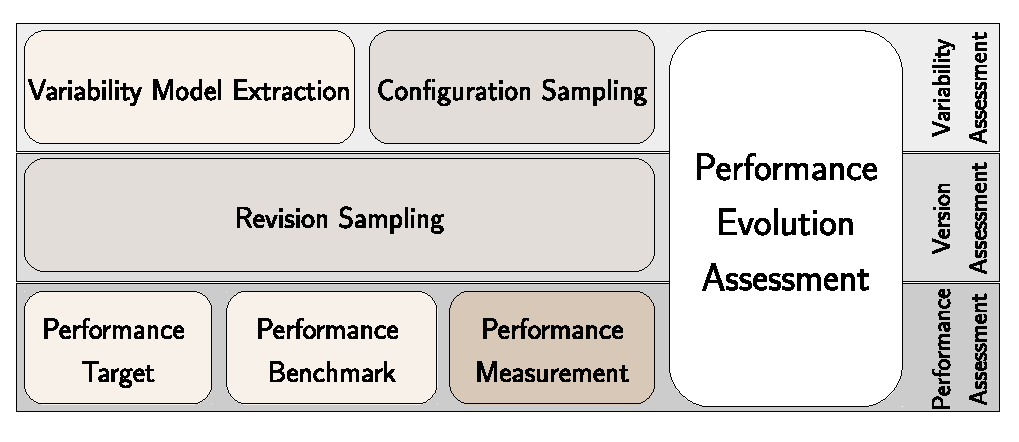
\includegraphics[width=0.75\textwidth]{images/process_overview.eps}
	\caption{Overview of the the proposed methodology including the necessary processes.}
	\label{fig:overview}
\end{figure}

First, objectives related to the variability of a configurable software system
are considered. This includes the extraction and comprehension of knowledge
about the system’s variability. Second, we address objectives which emerge with
evolving software, for instance whether a system compiles for a specific
version, or whether a version is a promising candidate for detecting
performance changes. Finally, we describe in detail the assessment of
performance which comprises the selection of suitable performance benchmarks as
well as a selection of appropriate statistical means to summarize, compare, and
evaluate performance statistics in order to derive meaningful insights.

In addition to the three aforementioned dimensions in Figure~\ref{fig:overview},
performance evolution assessment can also be conceived as consisting of three different
categories of tasks, as the different colorizations indicate. 
First, for a configurable software system, its variability needs to be
assessed in order to obtain a variability model to derive and
select configurations from.
Second, for a software system, a sample set of revisions needs to be selected.
Since covering all variants and versions is not feasible, a sampling strategy needs to be chosen
which is likely to uncover performance changes. Finally, the
performance assessment goals are specified and corresponding
measurements are conducted and evaluated as mentioned above.


\chapter{Background}\label{chapter:2}
This chapter is intended to recapitulate the background of the thesis theme. In
Sec.~\ref{sec:2.1}, we recall the evolution of software systems with respect to
architecture and variability. In Sec.~\ref{sec:2.2} we outline the characteristics
of software performance, practical testing and measurement strategies as well as
some statistical background necessary to analyze, interpret and compare
performance assessment. In Sec.~\ref{sec:2.3} we present recent approaches for
feature model extraction from existing software systems and code artifacts. Finally, in
Sec.~\ref{sec:2.4} we recall and compare in detail different approaches to model
and predict performance behavior for configurable software systems.

\section{Variability Modeling}
{\color{violet}
The design and development of configurable software systems is conceptually
divided into \emph{problem space} and \emph{solution space} \citep{czarnecki_generative_2000}. The problem space
comprises the abstract design of features that are contained in the software system as well as
constraints among features, such as dependencies or mutual-exclusion. The
solution space describes the technical realization of features and the
functionality described by and associated with features, e.g., implementation
and build mechanisms. That is, features cross both spaces since they are mapped
to corresponding code artifacts.}

A common way to express features and constraints in the problem space is to
define a \emph{variability model}, or \emph{feature model}, which subsumes all
valid configurations
\citep{kang_feature-oriented_1990,apel_feature-oriented_2013}. There are different and equivalent syntactical approaches to define feature models, for instance, a propositional formula $F$ over the set of
features of the configurable software systems \citep{batory_feature_2005}. In
this case a configuration is valid with respect to the feature model if and only if $F$ holds for all
selected features being true and all unselected features being false respectively. 
However, a more practical and more commonly used way to express feature models
are graphical tree-like \emph{feature diagrams}
\citep{apel_feature-oriented_2013}. In a feature diagram, features are ordered
hierarchically, starting with a root feature and subsequent child features. By
definition, the selection of a child feature requires the parent feature to be
selected as well. Child features can either be labeled as \emph{optional}
features  or \emph{mandatory} features; the latter ones need to be selected in
every valid configuration.
Moreover, feature diagrams
provide a syntax for two different types of feature groups, \emph{or-groups} or
\emph{alternative-groups}. For an or-group at least one of the group's features
needs to be selected for a valid configuration, whereas for an alternative group
exactly one out of the group's mutually exclusive features must be selected. In
addition to the feature hierarchy, constraints, which cannot be expressed by
the tree-like structure, are referred to as \emph{cross-tree constraints}.
Cross-tree constraints, depending on the notation, are depicted by arrows
between two features or simply added to the feature diagram as a propositional
formula. For such two features $f_1$ and $f_2$, a cross-tree constraint means
that for feature $f_1$ to be selected, either the selection of $f_2$ is
required/implied or excluded.

An introductory example for the syntax and semantics of feature diagrams is
provided in Fig.~\ref{fig:introduction_fm}. In this example an imaginary
vehicle propulsion can be configured with eight valid configurations. The vehicle requires an engine,
thus, feature \textsf{Engine} is mandatory. At least one out of the three
features \textsf{Hybrid}, \textsf{Piston} and \textsf{Electric} needs to be
selected. For a piston engine, we can select either the feature \textsf{Diesel}
or \textsf{Petrol}. A petrol engine requires additional ignition sparks in
contrast to a Diesel engine. For an electric engine we require a
battery, hence, the feature \textsf{Battery} is mandatory.
In addition, the feature model specifies two cross-tree constraints: First, the
feature \textsf{Tank} is optional, yet once a piston engine is selected, we
require  a tank. Second, if we want to use the \textsf{Hybrid} functionality
(e.g., use both electric and piston engine simultaneously), we require to have both a piston
and an electric engine.

\begin{figure}[htbp]
  \centering
  
  	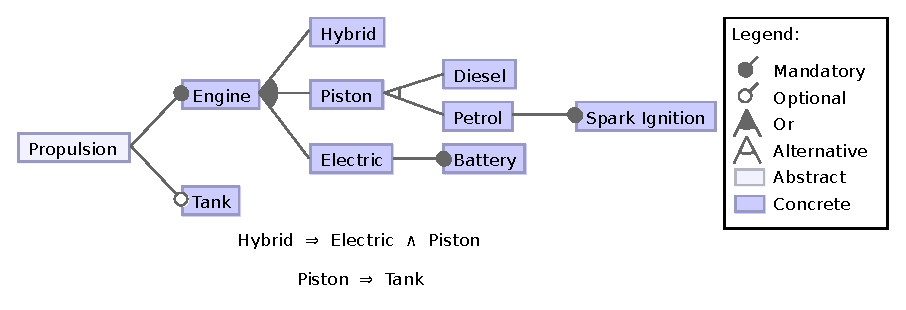
\includegraphics[width=0.85\textwidth]{images/introduction_fm.eps}
  \caption{Feature diagram for a feature model with eight valid configurations;
  two cross-tree constraints are specified as propositional formulas over
  features}
  \label{fig:introduction_fm}
\end{figure}

\section{Evolving Software} \label{sec:2.1}
\subsection{Software Evolution}
The first notion of a software systems' development process is usually
developer-centered and merely focuses on software being designed, implemented,
tested and eventually being released and deployed. Maintainability is a
generally recognized software quality property to look after, and maintenance
is, of course, essential to every successful software system. Nonetheless, less
attention is given to the ability to adapt a software system to changing
requirements (evolvability) rather than maintaining it to keep functionality
working \citep{parnas_software_1994}. Software evolution and evolvability, like
software itself are manifold. Software evolves in many ways ranging from maintenance (refactoring,
bug-fixes and patches) to adapting to changed requirements (adding, removing,
reorganizing functionality and variability).

Modern software systems not only often ship with a variety of configuration
options to select, they also employ routines to be build and sometimes even
make use of or are part of platforms, such as apps or plugins. That is,
software evolution affects all aforementioned aspects and maintainability as
well as evolvability can degrade as software evolves.

\subsection{Software Erosion}
The negative symptoms of software evolution, which are referred to as
``architectural erosion'' \citep{breivold_systematic_2012}, have
been addressed by many researchers.
Most of existing research so far though focuses on evolution regarding software architecture
\citep{breivold_systematic_2012}. The main driving factors leading to symptoms of decay
identified by \cite{perry_software_1991} are architectural erosion and
architectural drift. While architectural drift subsumes developers'
insensitivity when not following a systems architecture or respective guidelines while making changes, architectural erosion subsumes ignoring and violating the existing software
architecture. \cite{parnas_software_1994} argues that as software evolves, software is maintained
and evolved by developers who are not necessarily familiar with the initial
architectural design and, therefore, knowledge about the architecture becomes
unavailable. Although the unfavorable effects of software evolution do not necessary break a
system necessarily and imminently, the software becomes ``brittle'' \citep{perry_software_1991}
as maintainability as well as evolvability degrade. Concrete  symptoms of software
erosion on the implementation level have been documented. 

\cite{zhang_variability_2013} have studied erosion symptoms for a large-scale
industrial software product line with compile-time variability using
preprocessor directives.
They identify variability-related directives and clusters of those to tend to become more
complex as the software evolves. The negative effects, or symptoms of software
erosion are described as, but not limited to \emph{code replication} or
interdependencies between code elements, such as \emph{scattering} and
\emph{tangling}. Code scattering describes the phenomenon of code belonging to
a certain feature being scattered across multiple units of implementation,
e.g., modules, whereas code tangling means that code from different and
potentially unrelated features in entangled within a single module.

\cite{passos_feature_2015} have studied the extent of usage of scattering for device-drivers
in the Linux kernel. Despite scattering being quite prevalent, their
findings suggest that the kernel architecture is robust enough to have evolved
successfully. Nonetheless, platform drivers in the Linux kernel seem more
likely to be scattered than non-platform driver. They conclude that this is a
trade-off between maintainability and performance: a more generalized and
abstract implementation for platform-drivers in this case could possibly avoid
scattering, yet refactorings in this manner did not seem to be necessary or
worth the effort yet.

\subsection{Variability Evolution}
Apart from architecture evolution, the variability offered by software systems
evolves as well. For configurable software systems (or software product lines; 
these terms are not equivalent, but every SPL is a configurable software system)
evolution steps will not only affect artifacts in the solution space, yet also be visible in changes in the respective variability models.
Although the variability aspect of software evolution has not been drawn as
much attention to as has been on architecture in the past, more and more
research has emerged recently to address and understand variability evolution.

\cite{peng_analyzing_2011} proposed a classification of variability evolution patterns that
conceives evolution as adaption to changing (non-)functional requirements as
well as changing contexts. For a context in that sense, two
categories exist. A driving context determines, whether a variability model and respective variants
can meet functional requirements in the first place. A supporting context by
definition determines how non-functional properties are strengthened or
weakened. Any changed requirement is likely to change the contexts for a
software systems variability model and, therefore, will make adaptations of the
variability model necessary. Within their classification method Peng et al.
identify  major causes for variability evolution, comprising a) new driving
contexts emerging, b) weakened supporting contexts (for instance, due to new
non-functional requirements), and c) unfavorable trade-offs for non-functional
properties. 

To understand single evolutionary steps, several catalogs of variability
evolution patterns have been proposed. \cite{peng_analyzing_2011} present three patterns,
where either a new feature is added, a mandatory feature becomes optional, or a
mandatory/optional feature is split into alternative features. \cite{seidl_co-evolution_2012} suggest a catalog of
patterns for co-evolution of variability models and feature mappings that additionally introduces code clones, splitting a feature
into more fine-grained sub-features and feature removal as evolution patterns.
In addition, \cite{passos_towards_2012} have studied variability evolution in
the Linux kernel and present a catalog of patterns where features are removed from the
variability model, but remain a part of the implementation. Their
catalog, among others, includes feature merges, either implicit (optional feature merged
with its parent) or explicit.

The classification proposed by \cite{peng_analyzing_2011} is a general and formalized approach
that, as well as \cite{seidl_co-evolution_2012} and \cite{passos_towards_2012}, describes
elementary evolution patterns which can be composed to more complex patterns. Nonetheless, no
comprehensive catalog of variability evolution so far has been proposed as all
mentioned work above focuses on those patterns that appeared to be relevant for
the respective case study.

\section{Feature Model Synthesis}  \label{sec:2.3}
A variability model as an abstraction of functionality of a software system is
required, or at least of great interest, in many contexts. \emph{First}, not
every configurable system (or software product line) provides an explicit
representation of its variability model. 
The reasons for inexplicit or absent configuration specification are manifold.
They can range from poor or inconsistent documentation
\citep{rabkin_static_2011}, overly complex configurability \citep{xu_hey_2015}
or configuration constraints originated in different layers of a software
system, e.g.m build constraints  or compiler constraints \citep{nadi_where_2015}. 

\emph{Second}, variability models have emerged to be a useful means in domain
and domain analysis prior to developing a software system. As variability
models group and organize functionality, synthesizing a variability model has
shown to be applicable to extract features and constraints from functional
requirements. In addition, by comparison of product specifications for an
existing market domain, variability models can provide detailed feature summary.

For this thesis, we focus on the first aspect of synthesizing variability
models, as our work addresses the assessment of already existing configurable
software systems. Nonetheless, many techniques employed in the aforementioned
second aspect address similar problems, yet rely on natural language artifacts
rather than code artifacts \citep{alves_exploratory_2008,bakar_feature_2015}.
The following section recalls work on extracting configuration options and
constraints from source code as well as the organization of constraints into
feature hierarchy and groups. The further assessment of configurable systems
requires a well-defined and sound variability model.

\subsection{Feature Extraction} 
The first objective in recovering a variability model from a configurable
system is to determine the set of available configuration options to select. In
addition, for further configuration the type of each configuration option
(e.g., boolean, numeric or string) and the respective domain of valid values
needs to be specified.

\cite{rabkin_static_2011} proposed a static, yet heuristic approach to extract
configuration options along with respective types and domains. They exploit the
usage of configuration APIs. Their approach works
in two stages and commences with extracting all code sections where
configuration options are parsed. Subsequently, configuration names can be
recovered as they are either already specified at compile-time or can be
reconstructed using string analysis yielding respective regular expressions.
Moreover, they employ a number of heuristics to infer the type of parsed
configurations as well as respective domains. First, the return type of the
parsing method is likely to indicate the type of the configuration option read.
Second, if a string is read initially, the library method it is passed to can
reveal information about the actual type. For instance, a method
\emph{parseInteger} is likely to parse an integer value. Third, whenever a
parsed configuration option is compared against a constant, expression or value of an enum class,
these might indicate valid values or at least corner cases of the configuration
options' domain. The extraction method by \cite{rabkin_static_2011} renders to be precise, but is
limited, for instance, when an option leaves the scope of the source code.
Nonetheless, for the systems they evaluated they recovered configuration
options that were not documented, only used for debugging or even not used at
all.

\subsection{Constraint Extraction}
The second, or an additional step in recovering a variability model is the
extraction of configuration constraints. An approach proposed by \cite{zhou_extracting_2015}
focuses on the extraction of file presence conditions from build files using symbolic execution. A more comprehensive investigation of configuration
constraints and their origin is provided by \cite{nadi_mining_2014,nadi_where_2015}. They
propose an approach based on variability-aware parsing and infer constraints by
evaluating make files and  analyzing preprocessor directives. Inferred
constraints result from violations of two assumed rules, where a) every valid
configuration must not contain build-time errors and b) every valid
configuration should result in a lexically different program, thus. While the
first rule aims at inferring constraints that prevent build-time errors, the
second one is intended to detect features without any effect, at least as part
of some configurations. Their analysis one the one hand emerged to be accurate
in recovering constraints with 93~\% for constraints inferred by the first rule
and 77~\% for second one respectively. On the other hand, their approach was
only to recover 28~\% of all constraints present in the software system.
Further qualitative investigation, including developer interviews, lead to
the conclusion that most of existing constraints stem from domain knowledge.

\subsection{Feature Hierarchy Recovery} 
Besides recovering configuration options and respective constraints, to reverse
engineer a feature model, one further step is required. The recovered knowledge
needs a tree-like hierarchy, detection of feature groups and cross-tree
constraints to be an acceptable feature diagram
\citep{kang_feature-oriented_1990}. While several approaches to the recover feature model hierarchy have been proposed,
we are primarily interested in finding a hierarchy for knowledge obtained from
source code. Other scenarios, as already stated in the opener of this section,
are based on product descriptions or sets of valid configurations. The remainder of
this subsection we will focus on organizing features and constraints extracted
from source code. For further reading \cite{andersen_efficient_2012} present algorithms
for structuring feature diagrams for three different scenarios including the
ones previously mentioned.

Given an extracted set of features along with corresponding descriptions and
recovered constraints among the features, \cite{she_reverse_2011} propose an
semi-automated and interactive approach to synthesize a feature hierarchy.
Their approach comprises three steps: 1) Specifying a feature hierarchy, 2)
detecting and selecting feature groups, and 3) adding a cross-tree constraint
formula to the feature  model.

\begin{enumerate}
  \item Their approach commences with finding a single parent for each
  feature and, thus, specifying a tree-like feature hierarchy. Based on the
  given constraints a directed acyclic graph (DAG) representing implication
  relationships among features, a so-called implication graph, is constructed:
  Every vertex depicts a feature and edges are inserted for each pair of
  features $(u, v)$, where  $u \implies v$ holds with respect to the given
  constraints.
   
  In addition to the implication graph, the algorithm for each feature computes
  two rankings of features that are likely to be the respective parent feature.
  The two rankings both employ the feature descriptions. Feature descriptions
  are compared for similarity using a similarity metric. For two features $p$
  and $s$ the similarity is defined as the weighted sum of the inverse document
  frequencies $idf(w)$ for the words that the descriptions of features $u$ and
  $v$ share.
  The idf-ranking for a word $w$ is the logarithm of the number of features
  divided by the number of features whose description contains $w$. Each $idf$
  value is weighted by with by the frequency of $w$ in the description of
  feature $p$.
  
  The first ranking, called Ranked-Implied-Features (RIF), for each feature $f$
  ranks features by their similarity to $f$ in an descending order, but
  prioritizes those features that are implied according to the previously
  computed implication graph. The second ranking, called Ranked-All-Features
  (RAF) is similar to RIF, yet less strict since implied features are not
  prioritized. Given these ranking, a user selects for each feature a suitable
  parent feature from the RIF or RAF ranking. The idea behind providing two
  separate rankings, according to \cite{she_reverse_2011} is that the given
  extracted constraints can be incomplete and, thus, not all relevant implications are
  contained.

  \item After the feature hierarchy is specified, another auxiliary graph, a
  mutex graph, similar to the implication graph, is constructed. The mutex
  graph is an undirected graph with features as vertices and edges between two
  features $u$ and $v$, if $u \implies \neg{v}$ and $v \implies \neg{u}$ hold
  with respect to the given constraints. That is, all incident adjacent are mutually exclusive. Based on
  this mutex graph all maximal cliques (subsets of vertices that all are
  connected with each other) among the vertices with the same parent are
  computed. Those cliques are mutually exclusive and share the same parent and
  represent mutex- or alternative-groups. \cite{she_reverse_2011} introduce an
  additional constraint to extract xor-groups that require one of the groups’
  features to be selected if the parent is selected. This distinction is in
  line with the initial description of feature diagrams by \cite{kang_feature-oriented_1990},
  but not all descriptions follow this distinction between mutex- and
  xor-groups and just use the term alternative-group mentioned in Sec. 1.
  
  \item The cross-tree constraints for the feature diagram are extracted from
  the given configuration constraints. Since CTCs are constraints that could
  not be represented by the feature hierarchy (implication) or
  alternative-groups (exclusion) the derivation of CTCs follows this idea. The
  set of cross-tree implications is derived by removing all edges that are part
  of the feature hierarchy from the initially constructed implication graph.
  The set of cross-tree exclusions is derived in the same manner from the mutex
  graph by removing all edges among vertices of all mutex-groups. To make the
  feature model sound, the given configuration constraints, reduced to those
  clauses that are not already entailed by the diagram, can be added as an
  additional CTC formula to the feature diagram.
\end{enumerate}

The approach by \cite{she_reverse_2011} provides a practical algorithm to synthesize a
feature diagram, yet has some aspects we might need to consider. First, the
approach is not able to detect or-groups as defined in Sec. 1. Second, the
approach does introduce a root feature. Finally, the approach does not
distinguish between mandatory and optional features. Implicitly, all features
that do not have a parent feature are optional and all features that have a
parent feature are by default mandatory. \cite{she_reverse_2011} evaluated the
algorithm with both complete and incomplete variability knowledge (feature
names, descriptions and constraints). While the algorithm emerged to be
practical, detecting features whose parent was the root-feature was difficult.

\section{Assessing Performance} \label{sec:2.2}
While the last three sections covered software evolution and variability
modeling, we know step forward to the topic of software performance. This
section will the outline performance with respect to software systems as well
as to possible measurements. We provide a brief look at the general performance
testing setup and the required prerequisites, including suitable benchmarks.
Finally, we provide the statistical background to summarize, interpret and
compare performance measurements accurately.

\subsection{What is Performance?}
The performance of software systems is, like software quality, primarily a
matter of perspective. While an end user might consider practical aspects to be
more important, from a developer’s perspective, performance relates to and is
best described by non-functional properties \citep{molyneaux_art_2014}. While
functional properties subsume what exactly a software system does, non-functional
properties describe how (good or bad) a software system is at providing the
functionality offered. The notion of good and bad in this sense corresponds to
non-functional requirements (NFR), that is, software with good performance
behavior satisfies NFRs. The categories of NFRs what shape performance behavior
are manifold. According to \cite{molyneaux_art_2014}, \emph{key performance
indicators} (KPIs) include 

\begin{itemize}
  \item availability
  \item response time,
  \item resource utilization, and in a broader scope also 
  \item capacity.
\end{itemize}

Time-related KPIs are availability and response time, whereby
availability describes the time or time ratio that the software is available to
the end user and response time subsumes the time it takes to finish a request
or operation. Throughput as a category subsumes the program behavior with
respect to program load, such as hits per second for a web application or
amount of data processed per second. Resource utilization describes the extent
to which a software system uses the physical resources (CPU time, memory, and
disk or cache space) of the host machine. Finally, from a web-centered
perspective, capacity describes measurements with respect to servers and
networks, such as network utilization  (traffic, transmission rate) and server
utilization, such as resource limitations per application on a host server.

Consequently, the assessment of performance requires a context or testing
target that corresponds to the assesses system under test (SUT). For instance,
for a simple command-line compression tool, suitable KPIs are response time and
throughput, whereas performance for an online shop web application is better
outlined by availability and capacity.

\subsection{Performance and Software Engineering}
In the last section we referred to performance, or in detail, the KPIs, as
possible testing targets we validate against non-functional requirements.
However, in a broader sense software performance has become a facet of software
engineering and a lot of effort has been spent to study, describe, and improve
performance. Performance assessment in a software engineering context,
according to \cite{molyneaux_art_2014}, comprises a number of activities that
are related to or part of software development: Besides the analysis of concerns or
requirements with respect to performance, software performance engineering
entails performance testing and prediction and can contribute to maintenance
and evolution aspects \citep{woodside_future_2007}. While performance testing,
like other testing targets, is intended to validate requirements, prediction aims to
approximate performance behavior measures for different scenarios or
configurations. Moreover, performance behavior predictions can help anticipate
the impact of various changes \citep{woodside_future_2007}.
The authors, moreover, present the two approaches in assessing software
performance. So-called model-based approaches aim to describe performance
behavior by modeling functionality, for instance, modeling scenarios in UML,
using performance estimations early in the development process. In contrast to
that, accommodated later in the development process, measurement-based
approaches aim to model performance behavior based on measurements of existing
prototypes. The latter class of performance assessment includes classical
performance (regression) testing. The authors, moreover, outline the
anticipated future of both approaches and advocate the combination or
convergence of both approaches in the future. Since then, especially more
measurement-based performance prediction approaches have emerged. More on this
in the next section, the remainder of this subsection will outline the general
performance testing setup.

\subsection{Performance Testing}
The first step in performance testing, prior to defining relevant KPIs and
metrics, is to specify a system operation or use case \citep{woodside_future_2007} to
validate. A typical use case includes a well defined task or workload to
process, expected behavior or and outcome or state, and performance
requirements as previously discussed. For the SUT, however, we require a
version that does compile or, in case it is interpreted, is syntactically
correct \citep{molyneaux_art_2014}. With regard to performance assessments as part of
the development process, a code freeze should be obtained since measurement
results are likely to become meaningless for later versions. In addition to
that,  the machine or setup used for performance measurement should ideally be
as close to the production environment as possible, but at least be documented
to compare different runs.

Finally, one or more benchmarks need to be selected to simulate  the program
load for the respective use case. A benchmark, all in all, needs to be
representative, i.e., should relate to the the use case or requirement one
 wants to validate. While benchmarks for file compression usually include
multiple different types of media data (text, sound, pictures) like the
Canterbury corpus, web applications can be exposed to dealing with a number of
simulated users at the same time \citep{molyneaux_art_2014}. Benchmarks have often been
standardized within research and engineering to provide comparable performance
measurements. A popular examples is the Software Performance Evaluation
Corporation (SPEC), a consortium providing a variety of benchmarks like the
CPU2000 processor benchmark consisting of both floating point and integer
operations. Nonetheless, benchmarks in a sense of repeatable program load can
be obtained from load generation software like ApacheBench for the Apache web
server or simply by measuring performance for test cases.

Performance testing heavily relies on tool support, especially for repeating
test cases, recording measurements, and dynamic program analysis. While the
tool solutions for performance testing vary from domain, scale and purpose, we
will only outline the general tool architecture. \cite{molyneaux_art_2014} describes
four primary components: a scripting module, a test management module, a load
injector, and an analysis module. A scripting module handles the generation or
repetition of use cases which, for instance, can be recorded prior to the test
for web applications. A test management module creates and executes a test
session, whose program load is generated by one or more load injectors. A load
injector can provide a benchmark or generate items to process or can simulate a
number of clients for a server-side application. An analysis module, finally,
collects and summarizes data related to the performance testing target. More on
summarizing and comparing recorded results in the next section.

\subsection{Statistical Considerations}

\begin{itemize}
  \item Arithmetic mean: $$\text{a-mean} = \frac{1}{n}\sum_{i=1}^{n} X_i$$
  \item Geometric mean: $$\text{g-mean} = \bigg(\prod_{i=1}^{n}
  X_i\bigg)^\frac{1}{n} = \sqrt[\leftroot{-2}\uproot{2}n]{X_1 X_2 \ldots X_n}$$
  \item Harmonic mean: $$\text{h-mean} = n \cdot \bigg(\sum_{i=1}^{n}
  \frac{1}{X_i}\bigg)^{-1}$$
\end{itemize}

\section{Performance Modeling} \label{sec:2.4}
\begin{itemize}
  \item Genetic algorithms \citep{guo_genetic_2011}
  \item Variability-aware modeling \citep{guo_variability-aware_2013}
  \item via feature-interaction and performance influence models
  \citep{siegmund_predicting_2012,siegmund_performance-influence_2015}
\end{itemize}

\chapter{Performance Measurement Setup}\label{chapter:3}


\section{Performance Measurement Infrastructure}

\subsection{Repository Retrieval}
\subsection{Configuration Generation}
Prior to any test session, we require a set of valid configurations for the
configurable software system to benchmark. The configuraion semantics is
commonly expressed in feature diagrams (cf. Sect. 2), but can be translated to
and from propositional formulas or context-free grammars (CFGs) (although with
additional CTCs) as well \citep{batory_feature_2005}. The next section presents
a methodology to translate a given feature diagram to an equivalent CFG, derive
valid words from the CFG, and subsequently transform derived words to
configuration artifacts.

\begin{definition}[Context-free grammar]
A context-free grammar is a tuple $G = (N, T, S, P)$ with a set of non-terminal
symbols $N$, terminal symbols $T$, a start word $S \in (N \cup T)^*$, and set of
productions $P \subseteq N \times (N \cup T)^*$. 
\end{definition}

\begin{definition}[Configuration grammar]
A configuration grammar (CG) is a CFG, whereby all
features represent a non-terminal symbols. For each binary feature $b \in N$, we
introduce two terminal symbols $(b, 0)$ and $(b, 1)$. For each numeric feature
$n \in N$, we introduce as many terminal symbols of the form $(n, v)$ as
there are valid numeric values for $n$, where, $v \in dom(n)$. Based on the
feature hierarchy represented by the underlying feature diagram, we introduce a
production in the following manner. The set of productions is 

$$P_{CG} = \left\{ (p, \lbrace c \rbrace)~|~ p, c \in N \wedge p \implies  c
\right\} $$

\end{definition}

\begin{algorithm}[H]
 \KwData{this text}
 \KwResult{how to write algorithm with \LaTeX2e }
 initialization\;
 \While{not at end of this document}{
  read current\;
  \eIf{understand}{
   go to next section\;
   current section becomes this one\;
   }{
   go back to the beginning of current section\;
  }
 }
 \caption{How to write algorithms}
\end{algorithm}

\subsection{Sampling strategies}
\subsection{Benchmarks}
\subsection{Measurements with \texttt{GNU time}}
\subsection{Measurement Aggregation}



\section{Experiment Optimizations}

\section{Preprocessing Strategies}
\subsection{Variabilty Model Extraction}
\subsection{Build Mechnism Extraction}
\subsection{Release Commit Extraction}

\section{Case Study Corpus}

\chapter{Case Study Evaluation} \label{chapter:4} 
\chapter{Conclusion}\label{chapter:5}

\clearpage

%\addcontentsline{toc}{chapter}{Bibliography} 
\bibliography{library}

\end{document}
